\chapter{Common Knowledge}

\section{Motivating Example: The Corrupted Industry}

Consider an industry with 10 firms $C_1, C_2, \ldots, C_{10}$. Each firm $C_i$ has a manager $M_i$. The industry is thoroughly corrupted: every manager $M_i$ is secretly selling their own company's private information to all other companies. In addition, each company is buying private information from the managers of other companies.

\begin{center}
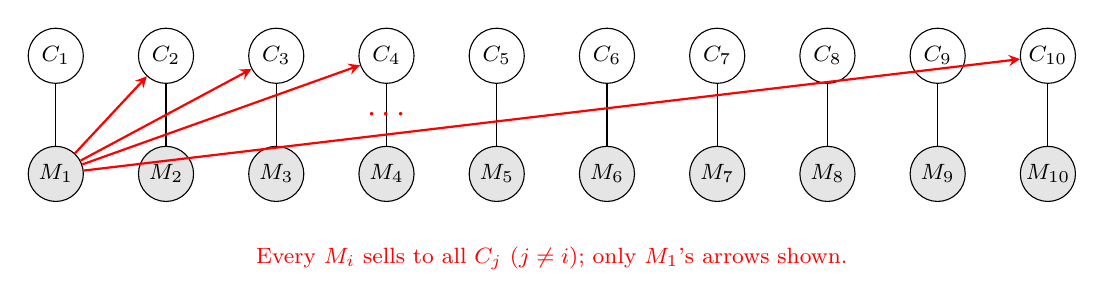
\begin{tikzpicture}[
  firm/.style={circle, draw, minimum size=7mm, inner sep=0pt, font=\footnotesize},
  mgr/.style={circle, draw, fill=gray!20, minimum size=7mm, inner sep=0pt, font=\footnotesize},
  >=stealth
]
  % Firms
  \foreach \i in {1,...,10} {
    \node[firm] (C\i) at ({(\i-1)*1.4}, 0) {$C_{\i}$};
  }
  % Managers
  \foreach \i in {1,...,10} {
    \node[mgr] (M\i) at ({(\i-1)*1.4}, -1.5) {$M_{\i}$};
  }
  % Vertical links (employment)
  \foreach \i in {1,...,10} {
    \draw (C\i) -- (M\i);
  }
  % M1 selling info: straight arrows to C2, C3, C4, dots, C10
  \draw[->, red, thick] (M1) -- (C2);
  \draw[->, red, thick] (M1) -- (C3);
  \draw[->, red, thick] (M1) -- (C4);
  \node[red, font=\large] at ({3*1.4}, -0.75) {$\cdots$};
  \draw[->, red, thick] (M1) -- (C10);
  
  % Note
  \node[below, font=\footnotesize, text=red, align=center] at ({4.5*1.4}, -2.3) {Every $M_i$ sells to all $C_j$ ($j \neq i$); only $M_1$'s arrows shown.};
\end{tikzpicture}
\end{center}

There is one corporate governance rule: if a company discovers that its own manager is selling information to outsiders, it will fire the manager on the \textbf{Friday of that week}.

\medskip
\noindent\textbf{What does each firm know?} Consider firm $C_1$. Since $C_1$ is buying information from the managers $M_2, M_3, \ldots, M_{10}$, it directly observes that those 9 managers are corrupt. However, $C_1$ \textbf{cannot observe whether its own manager $M_1$ is corrupt}---it does not know whether $M_1$ is selling to others. The same logic applies symmetrically to every firm. In summary:
\begin{itemize}
  \item Each firm knows that \textit{at least 9} managers are corrupt (the ones it buys from).
  \item No firm knows for certain whether its \textit{own} manager is corrupt.
\end{itemize}

Now suppose that at the start of Week 1, a regulator makes a \textbf{public announcement}: \textit{``At least one manager in this industry is corrupt.''} This statement is heard by all 10 firms simultaneously, and everyone knows that everyone heard it.

\medskip
\noindent\textbf{What happens?} Nothing happens in Week 1. Nothing happens in Week 2. In fact, nothing happens until \textbf{Week 10}, at which point all 10 managers are fired simultaneously.

\rmk{
  At first glance, this is deeply puzzling. Every firm already knew that at least 9 managers were corrupt---far more than the ``at least one'' in the announcement. How can such a seemingly vacuous statement trigger any action at all, let alone a cascade that takes 10 weeks to unfold?
}

\subsection{Iterated Reasoning}

The answer lies in the chain of \textit{iterated hypothetical reasoning} that the public announcement enables.

\medskip
\noindent\textbf{The $n = 1$ Case.}
Suppose there is only 1 firm with 1 corrupt manager.

\begin{center}
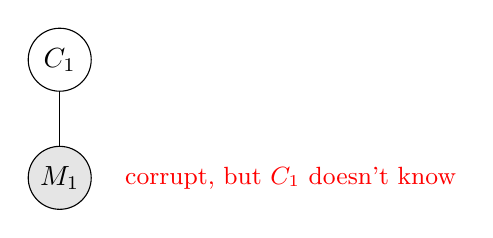
\begin{tikzpicture}[
  firm/.style={circle, draw, minimum size=8mm, inner sep=0pt},
  mgr/.style={circle, draw, fill=gray!20, minimum size=8mm, inner sep=0pt},
]
  \node[firm] (C1) at (0,0) {$C_1$};
  \node[mgr] (M1) at (0,-1.5) {$M_1$};
  \draw (C1) -- (M1);
  \node[right=3mm, font=\small, text=red] at (M1.east) {corrupt, but $C_1$ doesn't know};
\end{tikzpicture}
\end{center}

Before the announcement, $C_1$ does not know its own manager is corrupt. After the announcement (``at least one is corrupt''), $C_1$ immediately deduces that $M_1$ must be the corrupt one, and fires him on Friday of \textbf{Week 1}.

\medskip
\noindent\textbf{The $n = 2$ Case.}
Suppose there are 2 firms, both with corrupt managers. Each firm observes that the other firm's manager is corrupt (by buying information from him), but does not know about its own.

\begin{center}
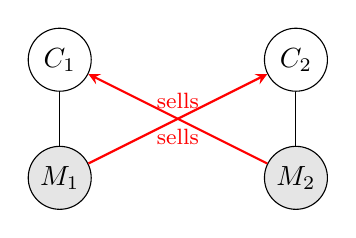
\begin{tikzpicture}[
  firm/.style={circle, draw, minimum size=8mm, inner sep=0pt},
  mgr/.style={circle, draw, fill=gray!20, minimum size=8mm, inner sep=0pt},
  >=stealth
]
  \node[firm] (C1) at (0,0) {$C_1$};
  \node[mgr] (M1) at (0,-1.5) {$M_1$};
  \node[firm] (C2) at (3,0) {$C_2$};
  \node[mgr] (M2) at (3,-1.5) {$M_2$};
  \draw (C1) -- (M1);
  \draw (C2) -- (M2);
  % Info selling
  \draw[->, red, thick] (M1) -- node[above, font=\footnotesize, text=red]{sells} (C2);
  \draw[->, red, thick] (M2) -- node[below, font=\footnotesize, text=red]{sells} (C1);
\end{tikzpicture}
\end{center}

Consider the reasoning from $C_1$'s perspective after the announcement. $C_1$ observes that $M_2$ is corrupt, but entertains two hypotheses about its own manager:
\begin{itemize}
  \item \textbf{Hypothesis A:} $M_1$ is not corrupt. Then only $M_2$ is corrupt. Under this hypothesis, after the public announcement, $C_2$ would find itself in the $n = 1$ situation: $C_2$ would see no other corrupt manager, learn from the announcement that at least one exists, and deduce that $M_2$ is the one. So $C_2$ would fire $M_2$ in \textbf{Week 1}.
  \item \textbf{Hypothesis B:} $M_1$ is also corrupt.
\end{itemize}
$C_1$ waits and watches. At the end of Week 1, $M_2$ is \textit{not} fired. This rules out Hypothesis A: if $M_1$ had been clean, $C_2$ would have acted already. Therefore $C_1$ concludes that $M_1$ must also be corrupt, and fires $M_1$ in \textbf{Week 2}.

By perfectly symmetric reasoning, $C_2$ also watches whether $C_1$ fires $M_1$ in Week 1. When it does not happen, $C_2$ likewise infers that $M_2$ is corrupt. Both managers are fired simultaneously in \textbf{Week 2}.

\medskip
\noindent\textbf{The General Case: Induction.}
By induction on the number of corrupt managers $n$. Each firm sees $n - 1$ corrupt managers and entertains the hypothesis that its own manager is clean (so that only $n - 1$ managers are corrupt). Under that hypothesis, by the inductive assumption, the other $n-1$ firms would have fired their managers by Week $n - 1$. When this does not happen by the end of Week $n - 1$, every firm deduces that the total must be $n$, meaning its own manager is also corrupt. All $n$ managers are fired simultaneously in \textbf{Week $n$}.

For our example with $n = 10$: nothing happens for 9 weeks, and then all 10 managers are fired in Week 10.

\subsection{Why Does a ``Vacuous'' Announcement Matter?}

The content of the announcement (``at least one is corrupt'') was already known to every firm---each firm could see at least 9 corrupt managers. What was \textit{not} in place before the announcement was the full tower of \textit{hypothetical reasoning about hypothetical reasoning}.

To see why, trace the chain from $C_1$'s perspective. $C_1$ reasons: ``I see 9 corrupt managers. But suppose $M_1$ is clean. Then $C_2$ would see only 8 corrupt managers. And $C_2$ might suppose $M_2$ is also clean. Then $C_3$ would see only 7\ldots'' Each level of nesting reduces the number of known-corrupt managers by one. After 9 levels of hypothetical reasoning, we reach a scenario where some firm sees \textit{zero} other corrupt managers and does not know if any exist at all. Without the announcement, the induction has no base case in this deepest hypothetical---the chain of reasoning collapses before reaching its logical conclusion.

The public announcement plugs exactly this gap. By making ``at least one is corrupt'' publicly and simultaneously known to all, it provides the base case in every hypothetical scenario, no matter how deeply nested. This distinction---between knowledge that is shared but \textit{finitely} nested, and knowledge that is shared \textit{infinitely} deep---is precisely the distinction between \textit{mutual knowledge} and \textit{common knowledge}, which we now formalize.

\section{Formal Definition}

\defn{Mutual Knowledge and Common Knowledge}{
  Let $E$ be an event and let there be $n$ agents.
  \begin{itemize}
    \item $E$ is \textbf{mutual knowledge of order 1} if every agent knows $E$.
    \item $E$ is \textbf{mutual knowledge of order $k$} if every agent knows that $E$ is mutual knowledge of order $k - 1$.
    \item $E$ is \textbf{common knowledge} if $E$ is mutual knowledge of order $k$ for \textit{every} $k \in \mathbb{N}$.
  \end{itemize}
  In other words, common knowledge means: everyone knows $E$, everyone knows that everyone knows $E$, everyone knows that everyone knows that everyone knows $E$, and so on \textit{ad infinitum}.
}

In the corrupted industry example, the event $E = $ ``at least one manager is corrupt'' was, before the announcement, mutual knowledge of high order but \textbf{not} common knowledge. Each firm's chain of hypotheticals (``suppose mine is clean, then you see one fewer, then suppose yours is clean too\ldots'') bottoms out after finitely many levels at a scenario in which one firm sees zero corrupt managers and cannot determine whether $E$ holds. Common knowledge requires that the chain never bottoms out---that at every depth of hypothetical reasoning, every agent in the hypothetical scenario still knows $E$.

The public announcement achieves exactly this. Because every firm heard the announcement, and every firm knows every other firm heard it, and so on without bound, $E$ becomes common knowledge. The base case of the induction (``a firm that sees zero corrupt managers and hears the announcement will fire its manager in Week 1'') is now available at every depth, enabling the full chain of iterated reasoning to unfold.

\section{The Coordinated Attack Problem}

We now present a game-theoretic example that dramatically illustrates the difference between ``almost common knowledge'' and true common knowledge. This is based on Rubinstein's (1989) \textit{Electronic Mail Game}.

\subsection{Setup}

Two divisions of an army (Player 1 and Player 2) must decide whether to \textbf{attack} ($A$) or \textbf{not attack} ($N$). The enemy is either \textbf{weak} (state $G$, the ``good'' state) or \textbf{strong} (state $B$, the ``bad'' state). The army wins if and only if \textit{both} divisions attack \textit{and} the enemy is weak. The prior probabilities are $\Pr{G} = \pi < \frac{1}{2}$ and $\Pr{B} = 1 - \pi$.
\todo{learn how the command ``Pr'' is defined in the file commands.tex. and revise those for all the remaining Pr's. Also, if you find my current redefinition of Pr is not that appropriate, tell me and advise me how to revise it.}
The payoff matrices are:

\begin{center}
\begin{tabular}{cc}
\textbf{State $G$} (prob $\pi$) & \textbf{State $B$} (prob $1-\pi$) \\[6pt]
$\begin{array}{c|cc}
 & A & N \\ \hline
A & 2,\;2 & -3,\;0 \\
N & 0,\;-3 & 0,\;0
\end{array}$
&
$\begin{array}{c|cc}
 & A & N \\ \hline
A & -2,\;-2 & -2,\;0 \\
N & 0,\;-2 & 0,\;0
\end{array}$
\end{tabular}
\end{center}

In state $B$, not attacking ($N$) is strictly dominant for both players. In state $G$, the game is a \textit{coordination game}: $(A, A)$ is a Nash equilibrium with payoff $(2,2)$, but attacking alone is severely punished ($-3$). Crucially, if the state $G$ were \textbf{common knowledge}, both $(A, A)$ and $(N, N)$ would be Nash equilibria---the game is a coordination game with two pure-strategy equilibria. The interesting question is whether the players can coordinate on the Pareto-superior equilibrium $(A, A)$.

\subsection{Information Structure}

The communication protocol is as follows:
\begin{enumerate}
  \item If the state is $G$, Nature sends a signal to Player 1 with certainty (no error at this stage). If the state is $B$, no signal is sent.
  \item Upon receiving a signal, Player 1's system \textit{automatically} forwards a message to Player 2. This transmission fails (the message is lost) with probability $\ve > 0$, independently.
  \item If Player 2 receives the message, Player 2's system automatically sends a confirmation back to Player 1, again lost with probability $\ve$.
  \item This back-and-forth continues indefinitely: each successfully received message triggers an automatic reply, each of which is independently lost with probability $\ve$.
\end{enumerate}
The message sending is \textit{not} a strategic choice---it is automatic. The only strategic decision is whether to attack or not.

Let $t_i$ denote the \textbf{number of messages received} by Player $i$. In state $B$, no messages are sent, so $t_1 = t_2 = 0$. In state $G$, the message chain proceeds as:
\begin{center}
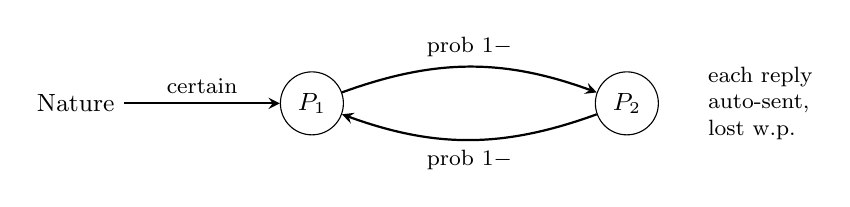
\begin{tikzpicture}[>=stealth, font=\small]
  \node (N) at (-2, 0) {Nature};
  \node[draw, circle, minimum size=8mm] (P1) at (1, 0) {$P_1$};
  \node[draw, circle, minimum size=8mm] (P2) at (5, 0) {$P_2$};
  
  \draw[->, thick] (N) -- node[above]{\footnotesize certain} (P1);
  \draw[->, thick, bend left=20] (P1) to node[above]{\footnotesize prob $1-\ve$} (P2);
  \draw[->, thick, bend left=20] (P2) to node[below]{\footnotesize prob $1-\ve$} (P1);
  
  \node[right=5mm, align=left, font=\footnotesize] at (P2.east) {each reply\\auto-sent,\\lost w.p.\ $\ve$};
\end{tikzpicture}
\end{center}

The chain stops at the first lost message. The possible outcomes given state $G$ are:
\begin{center}
\renewcommand{\arraystretch}{1.1}
\begin{tabular}{ccc}
  Chain stops at & $t_1$ & $t_2$ \\
  \hline
  $P_1 \to P_2$ lost & $1$ & $0$ \\
  $P_2 \to P_1$ lost & $1$ & $1$ \\
  $P_1 \to P_2$ lost & $2$ & $1$ \\
  $P_2 \to P_1$ lost & $2$ & $2$ \\
  $\vdots$ & $\vdots$ & $\vdots$ \\
\end{tabular}
\end{center}
Observe that $t_1$ and $t_2$ always differ by at most 1: given $t_1 = T \ge 1$, the value of $t_2$ is either $T - 1$ or $T$.

\rmkb[``Almost'' Common Knowledge]{
  When $\ve$ is small, the message chain is very likely to be long. With high probability, both players receive many confirmations, so each player is ``almost sure'' the state is $G$, ``almost sure'' the other knows it, ``almost sure'' the other knows the other knows it, and so on. The state $G$ is ``almost'' common knowledge. One might expect that $(A, A)$ should be sustainable as an equilibrium. As we will see, this intuition is spectacularly wrong.
}

\subsection{The Unique Equilibrium}


A strategy for Player $i$ is a function $\sigma_i: \{0, 1, 2, \ldots\} \to \{A, N\}$ mapping the number of messages received to an action.

\prop{Unique Equilibrium of the Coordinated Attack Game}{
  There is a unique equilibrium: both players play $N$ regardless of the number of messages received. That is, $\sigma_i(t_i) = N$ for all $t_i \ge 0$ and $i \in \{1, 2\}$.
}
\begin{proppf}
  By induction on the number of messages received.
  
  \medskip
  \noindent\textbf{Base case: $t_1 = 0$.} If Player 1 receives no messages, then state $B$ is certain (since Nature always signals Player 1 in state $G$). In state $B$, $N$ is strictly dominant. So $\sigma_1(0) = N$.
  
  \medskip
  \noindent\textbf{Base case: $t_2 = 0$.} If Player 2 receives no messages, there are two possibilities:
  \begin{enumerate}[label=(\roman*)]
    \item State is $B$ and no signal was ever sent (prior probability $1 - \pi$);
    \item State is $G$, Player 1 received the signal, but the forward to Player 2 was lost (prior probability $\pi\ve$).
  \end{enumerate}
  By Bayes' rule:
  \[
  \Pr{G \mid t_2 = 0} = \frac{\pi\ve}{\pi\ve + (1 - \pi)}.
  \]
  If Player 2 plays $N$, the payoff is 0. If Player 2 plays $A$, the payoff is at most (assuming Player 1 plays $A$ whenever state is $G$):
  \[
  \Pr{G \mid t_2 = 0} \times 2 + \Pr{B \mid t_2 = 0} \times (-2) = \frac{2\pi\ve - 2(1 - \pi)}{\pi\ve + (1 - \pi)} < 0,
  \]
  since $\pi\ve \ll 1 - \pi$ (recall $\pi < \frac{1}{2}$ and $\ve$ is small). So $\sigma_2(0) = N$.
  
  \medskip
  \noindent\textbf{Inductive step.} Suppose that for all $t_1, t_2 < T$, both players play $N$: $\sigma_1(t_1) = N$ and $\sigma_2(t_2) = N$.
  
  Consider Player 1 with $t_1 = T$ (the argument for Player 2 is symmetric). Given $t_1 = T$, Player 2's message count is either $t_2 = T - 1$ or $t_2 = T$. The conditional probability is:
  \[
  p := \Pr{t_2 = T - 1 \mid t_1 = T} = \frac{\ve}{\ve + (1-\ve)\ve} = \frac{1}{2 - \ve} > \frac{1}{2}.
  \]
  This is because, given $t_1 = T$: with probability $\ve$ the next message ($P_1 \to P_2$) is lost, yielding $t_2 = T-1$; with probability $(1-\ve)\ve$ the message reaches $P_2$ (so $t_2 \ge T$) but the return is lost, yielding $t_2 = T$.
  
  By the induction hypothesis, $\sigma_2(T-1) = N$. Even in the best case where Player 2 plays $A$ when $t_2 = T$, if Player 1 plays $A$:
  \[
  \text{Payoff to } P_1 \le p \times (-3) + (1 - p) \times 2 = \frac{-3 + 2(1 - \ve)}{2 - \ve} = \frac{-1 - 2\ve}{2 - \ve} < 0.
  \]
  The $-3$ arises because when $t_2 = T-1$, Player 2 plays $N$ (by induction), so Player 1 attacks alone. The $2$ is the best-case payoff if Player 2 also attacks. Since $p > \frac{1}{2}$, the expected payoff from attacking is strictly negative. Therefore $\sigma_1(T) = N$.
  
  By symmetric reasoning applied to Player 2, $\sigma_2(T) = N$. This completes the induction.
\end{proppf}

\subsection{Interpretation}

The result is striking. The following two scenarios yield completely different equilibrium outcomes:

\begin{center}
\renewcommand{\arraystretch}{1.3}
\begin{tabular}{ll}
  \textbf{Information structure} & \textbf{Equilibrium outcome} \\
  \hline
  $G$ is \textbf{common knowledge} & $(A, A)$ is a NE \\
  $G$ is ``almost'' common knowledge & $(N, N)$ is the \textit{unique} NE
\end{tabular}
\end{center}

No matter how small $\ve > 0$ is, and no matter how many thousands of confirmations each player has received, the \textit{unique} equilibrium is for both to play $N$. The problem is not that the players lack confidence that $G$ is true---after many messages, they are nearly certain. The problem is that each player is never quite sure the \textit{other} player is sure that the other player is sure\ldots\ that the state is $G$.

\rmkb[Common $p$-Belief]{
  The key quantitative insight is the conditional probability $p = \frac{1}{2-\ve}$. Even when $\ve$ is tiny, $p$ is close to $\frac{1}{2}$---far from 1. This means that no matter how many messages Player $i$ has received, Player $i$ always assigns probability at least $\frac{1}{2}$ to the event that the other player received one fewer message. The information structure ``self-replicates'' at every level: the uncertainty never shrinks as we go deeper in the epistemic hierarchy.
  
  This connects to the concept of \textit{common $p$-belief} (Monderer and Samet, 1989): an event is common $p$-belief if everyone believes it with probability at least $p$, everyone believes with probability at least $p$ that everyone believes it with probability at least $p$, and so on. In the electronic mail game, the state $G$ is common $p$-belief only for $p \le \frac{1}{2-\ve} \approx \frac{1}{2}$, which is far from the $p = 1$ required for common knowledge. Coordination requires common knowledge (or at least common $p$-belief with $p$ sufficiently large); ``almost common knowledge'' is not enough.
}









